\newlecture

\setcounter{chapter}{12}
\setcounter{section}{0}

\def\textbookchapter{Course Topic IV: Vector Calculus}
\def\coursetopicnumber{IV}
\def\topic{Vector Fields} % this is the printed title
\def\shorttopic{Vector fields} % short topic
\def\textbookname{Active Calculus} % this is the corresponding textbook
\def\shorttextbookname{AC} % this is the short name for the book
\def\textbooksection{12.1} % corresponding textbook section
\def\textbooksectionurl{https://activecalculus.org/vector/S_Vector_VectorFields.html} % URL for textbook section
\def\handoutday{} % this is the printed date

\addtocontents{toc}{\bigskip \large \textbookchapter \normalsize \medskip \par} %% for table of contents
%%%%%%%%% DOCUMENT CONTENT STARTS BELOW

\thispagestyle{plain}
\topstuff
\section{\topic{} \booklink{}}
\label{sec:vector-fields}
\subsection{Definition and visualization}
Vector fields are ubiquitous in everyday life. We experience them as gravitational fields, electric fields, force fields, fluid flow, wind flow, and so on.

\begin{defn}[Vector Field]
    A \emph{vector field} is a function that takes points as input and gives vectors as output. If the input point is in $\mathbb{R}^n$, then the vector also has $n$ components.
\end{defn}

\begin{example}
    Here are a few examples in 2 and 3 dimensions.
    \begin{multicols}{2}
        \begin{itemize}
            \item $\vec{F}(x,y)=\langle x,\, y\rangle$
            \item $\vec{F}(x,y)=\langle x^2-y^2,\, 0\rangle$
            \item $\vec{F}(x,y,z)=\langle xy,\,  yz,\,  4+x+y\rangle$
            \item $\vec{F}(x,y,z)=\langle 1,\,  2,\,  e^z\rangle$
        \end{itemize}
    \end{multicols}
\end{example}

To visualize a vector field $\vec{F}(x,y)$, do the following:
\begin{itemize}
    \item create a grid of sample points;
    \item at each sample point $P=(x,y)$ (or $P=(x,y,z)$), draw the vector $\vec{F}(P)$ with its tail at $P$.
\end{itemize}

\begin{example}
    Here are a few graphical representations of 2D vector fields.
    \\
    \begin{minipage}{.4\textwidth}
        \begin{center}
            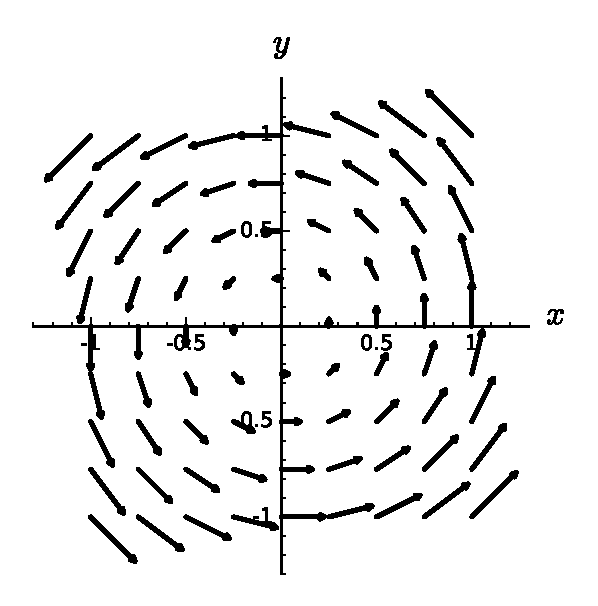
\includegraphics[width=.9\textwidth]{images/vf1.eps}\label{img:sage-vector-field-1} \medskip 
            
            $\vec{F}(x,y) = \left\langle -\dfrac{y}{4}, \, \dfrac{x}{4}\right\rangle$ 
        \end{center}
    \end{minipage}
    \hfill 
    \begin{minipage}{.4\textwidth}
        \begin{center}
            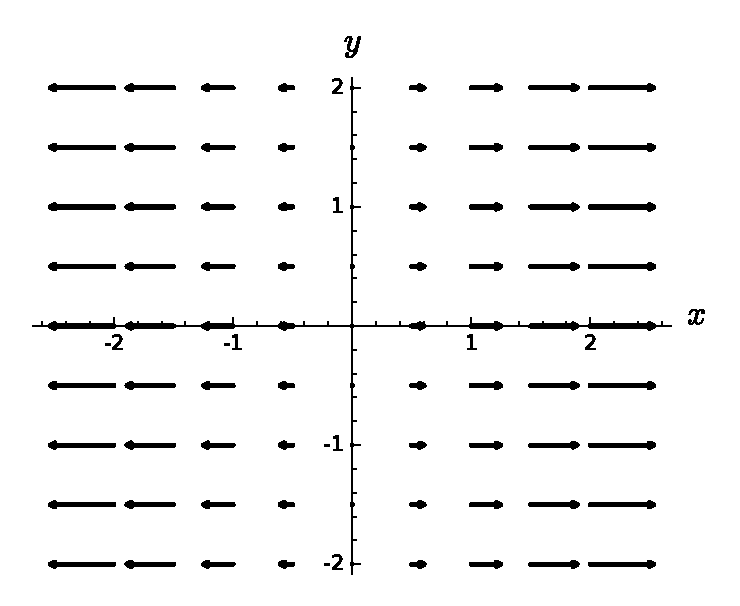
\includegraphics[width=.9\textwidth]{images/vf2.eps} \medskip
            
            $\vec{F}(x,y) = \left\langle \dfrac{x}{3}, \, 0\right\rangle$ 
        \end{center}
    \end{minipage}
\end{example}

We can view a vector field as a velocity field, where each arrow represents a velocity vector (with a direction and a magnitude).

\begin{defn}[Flow curve, stream line]
    A path that follows the directions of a vector field is called a \emph{flow curve} or \emph{stream line}.
\end{defn}
%\pagebreak 

\begin{ex}
    On the axes below, sketch the vector field  $\vec{F}(x,y)=\langle y,\,  -x \rangle$.
    
    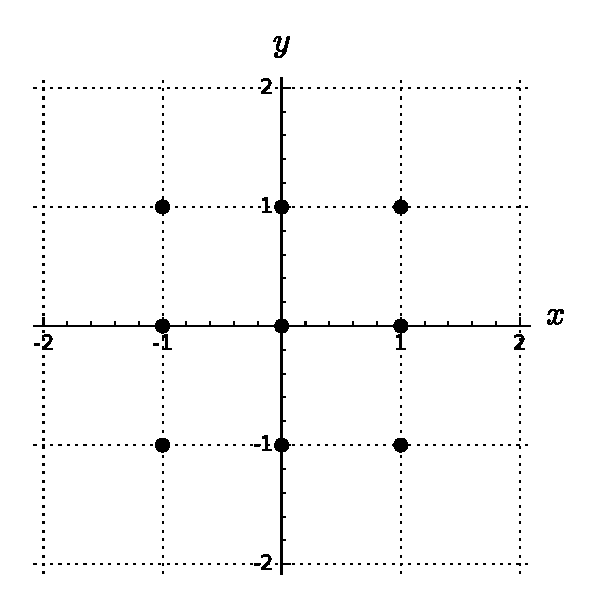
\includegraphics[width=.5\textwidth]{images/dots_fewer}
\end{ex}

\vfill 

\begin{ex}
    On the axes below, sketch the vector field   $\vec{F}(x,y)=\dfrac{1}{2}\vec{i}+\dfrac{x}{2}\vec{j}$.

    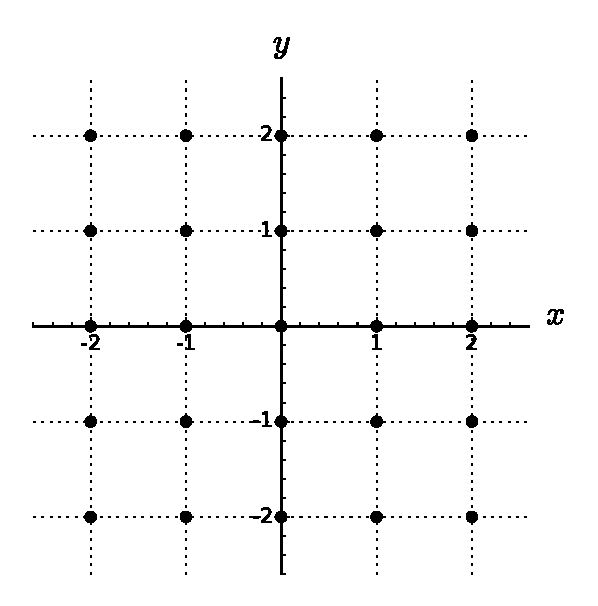
\includegraphics[width=.5\textwidth]{images/dots_more}
\end{ex}

\pagebreak 

\begin{ex}
    Identify the following vector fields with the sketches below. (Some are scaled a bit to avoid overlapping arrows.)
    \begin{multicols}{4}
    \begin{enumerate}
        \item $\vec{F}=\langle 0,\, x^2\rangle$
        \item $\vec{F}=\langle y,\, x\rangle$
        \item $\vec{F}=\langle 2x,\, -y\rangle$
        \item $\vec{F}=\langle x-y,\, x\rangle$
    \end{enumerate}
    \end{multicols}
    
    \begin{minipage}{.4\textwidth}
        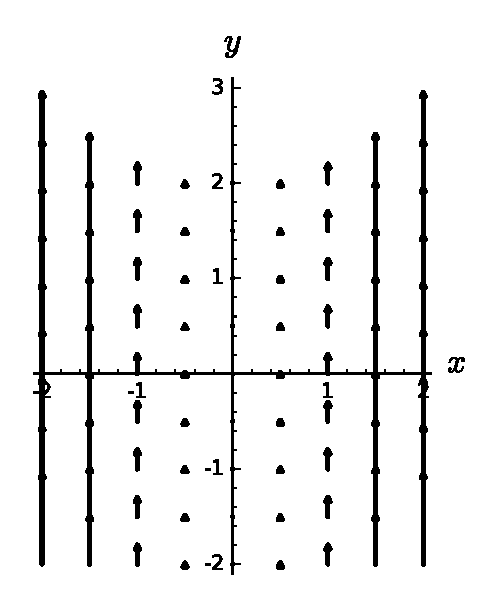
\includegraphics[width=\textwidth]{images/mult1} \label{img:sage-vector-field-2}
    \end{minipage}
    \hfill
    \begin{minipage}{.4\textwidth}
        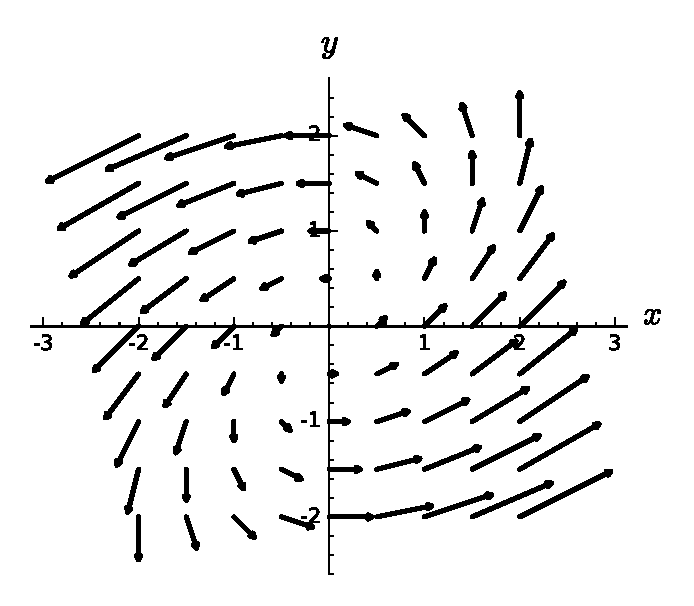
\includegraphics[width=\textwidth]{images/mult2}
    \end{minipage}
    
    \begin{minipage}{.4\textwidth}
        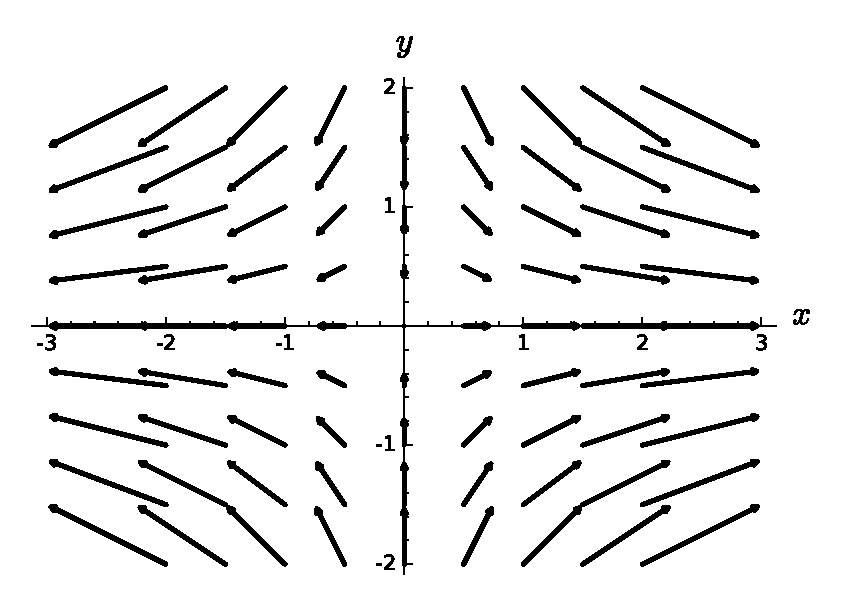
\includegraphics[width=\textwidth]{images/mult3}
    \end{minipage}
    \hfill
    \begin{minipage}{.4\textwidth}
        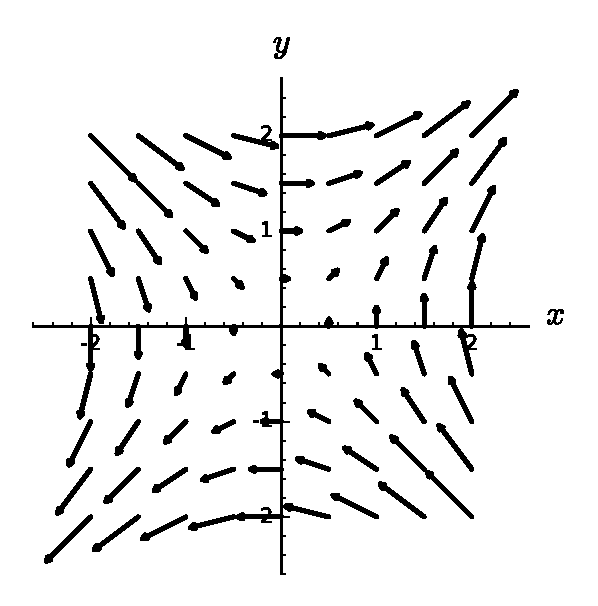
\includegraphics[width=\textwidth]{images/mult4}
    \end{minipage}
\end{ex}

\subsection{Gradient vector fields}
We learned about the gradient of a multivariable function in Chapter 10. Recall the following.
\begin{defn}[Gradient]
    The \emph{gradient} of a scalar-valued function is a vector-valued function:
    \[
        \nabla f(x,y)=\phantom{\langle f_x(x,y),\, f_y(x,y)\rangle}
    \] 
    and 
    \[
        \nabla f(x,y,z)=\phantom{\langle f_x(x,y,z),\, f_y(x,y,z),\, f_z(x,y,z)\rangle.}
    \]
\end{defn}
\vfill 

\noindent Thus, for any multivariable function $f$ we have a corresponding vector field $\nabla f$.

\pagebreak 

\begin{ex}
    For $f(x,y,z)=xyz$, compute the vector field $\nabla f(x,y,z)$.
\end{ex}\vspace{1in}

\begin{ex}
    For $f(x,y)=x^2+y^2$, sketch the vector field $\nabla f(x,y)$ on a $3\times3$ grid of points around the origin.
\end{ex}

\vspace{1.6in}

\subsection{Potential functions}
\begin{defn}[Gradient field, potential function]
    Given a vector field $\vec{F}$, if $\vec{F}$ is the gradient of some scalar function $f$, then we call $\vec{F}$ a \emph{gradient field} and we say $f$ is a \emph{potential function} for $\vec{F}$.
    
    In other words, if $\vec{F}=\nabla f$, then $\vec{F}$ is a gradient vector field with potential function $f$.
\end{defn}

\bigskip

\vspace{.6in}

\begin{ex}\label{ex:first-search-for-potential-fns}
    Find a potential function, if one exists, for each vector field.
    \begin{multicols}{4}
    \begin{enumerate}
        \item \mbox{$\vec{F}(x,y)=\langle 2x,\,2y\rangle$}
        \item \mbox{$\vec{F}(x,y)=\langle 2y,\,2x\rangle$}
        \item \mbox{$\vec{F}(x,y)=\langle x,\,3\rangle$}
        \item \mbox{$\vec{F}(x,y)=\langle y,\,3\rangle$}
    \end{enumerate}
    \end{multicols}
     %$\vec{F}(x,y,z)=\langle x+y, x+z, y+z\rangle$.
\end{ex}

\vfill


